\documentclass[tikz,border=10pt]{standalone}

\usepackage{amsmath,amssymb}
\usepackage{tikz}
\usetikzlibrary{arrows.meta,positioning,calc,fit}

\newcommand{\C}{\mathbb{C}}

\begin{document}
	
	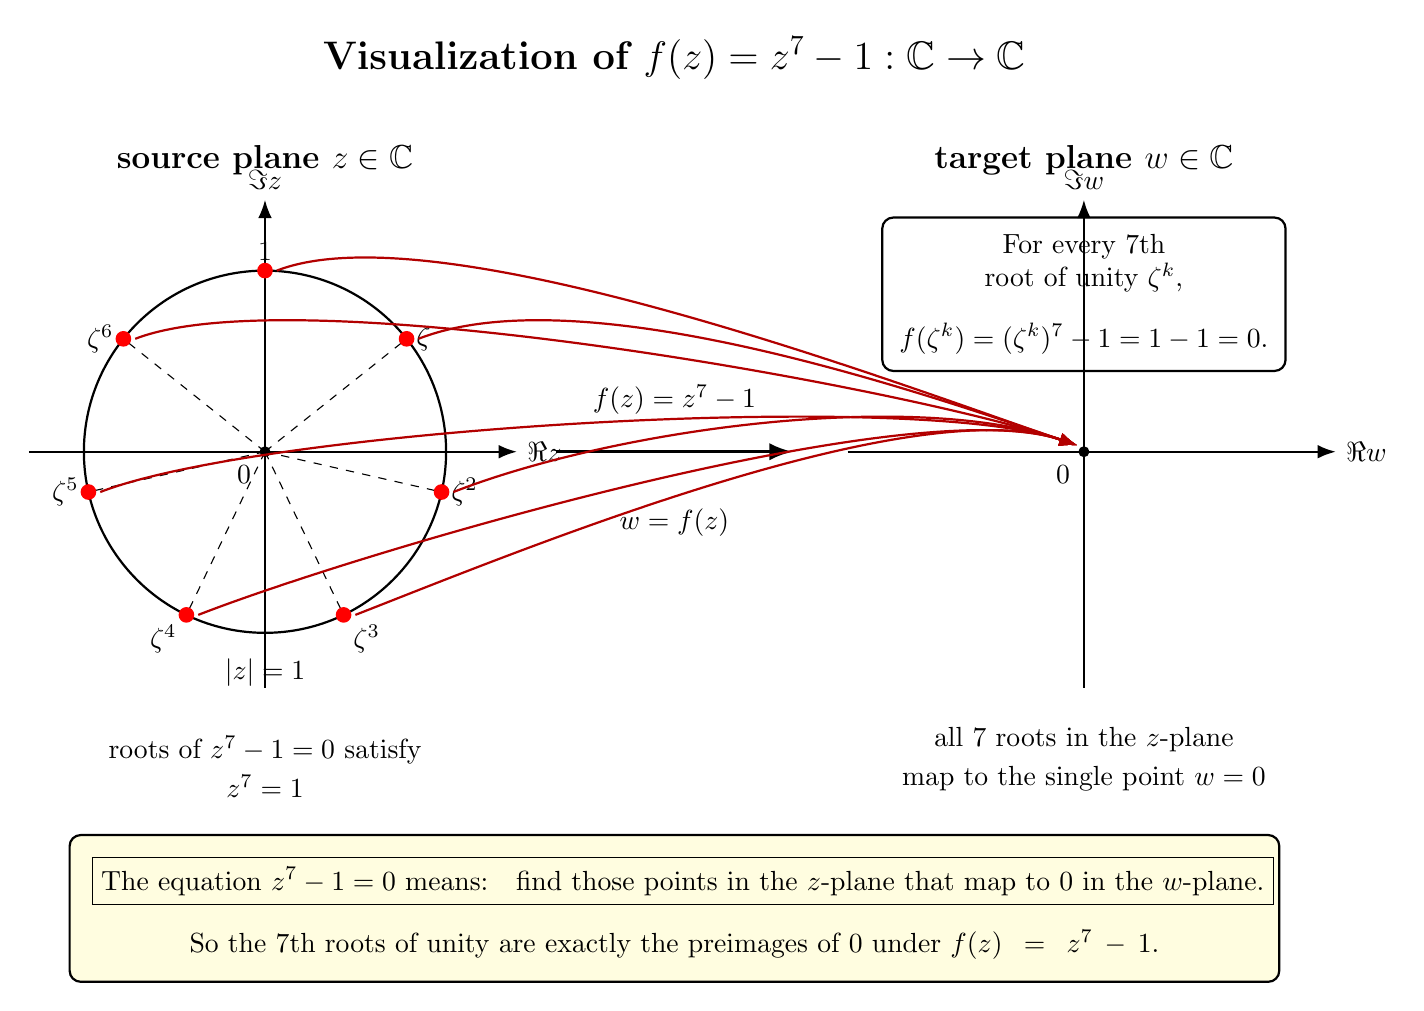
\begin{tikzpicture}[
		>=Latex,
		axis/.style={thick},
		root/.style={circle, fill=red, inner sep=2pt},
		pt/.style={circle, fill=black, inner sep=1.4pt},
		box/.style={draw, rounded corners, thick, align=center, inner sep=6pt}
		]
		
		% --------------------------------------------------
		% Title
		% --------------------------------------------------
		\node[font=\bfseries\Large] at (0,5.2)
		{Visualization of $f(z)=z^7-1:\C\to\C$};
		
		% --------------------------------------------------
		% Left plane: z-plane
		% --------------------------------------------------
		\coordinate (L) at (-5.2,0.2);
		
		\node[font=\bfseries\large] at ($(L)+(0,3.7)$) {source plane $z\in\C$};
		
		% axes
		\draw[axis,->] ($(L)+(-3.0,0)$) -- ($(L)+(3.2,0)$) node[right] {$\Re z$};
		\draw[axis,->] ($(L)+(0,-3.0)$) -- ($(L)+(0,3.2)$) node[above] {$\Im z$};
		
		% unit circle
		\draw[thick] (L) circle (2.3cm);
		\node at ($(L)+(0,-2.8)$) {$|z|=1$};
		
		% origin
		\node[pt,label=below left:$0$] at (L) {};
		
		% 7 roots
		\foreach \k/\ang in {0/90,1/38.571,2/-12.857,3/-64.286,4/-115.714,5/-167.143,6/141.429}
		{
			\coordinate (P\k) at ($(L)+(\ang:2.3cm)$);
			\draw[dashed] (L) -- (P\k);
			\node[root] at (P\k) {};
		}
		
		% labels
		\node[above] at (P0) {$1$};
		\node[right] at (P1) {$\zeta$};
		\node[right] at (P2) {$\zeta^2$};
		\node[below right] at (P3) {$\zeta^3$};
		\node[below left] at (P4) {$\zeta^4$};
		\node[left] at (P5) {$\zeta^5$};
		\node[left] at (P6) {$\zeta^6$};
		
		\node[align=center] at ($(L)+(0,-4.0)$) {%
			roots of $z^7-1=0$ satisfy\\[2pt]
			$z^7=1$
		};
		
		% --------------------------------------------------
		% Middle arrow
		% --------------------------------------------------
		\draw[->, very thick] (-1.5,0.2) -- (1.5,0.2);
		\node[above, align=center] at (0,0.55) {$f(z)=z^7-1$};
		\node[below, align=center] at (0,-0.4) {$w=f(z)$};
		
		% --------------------------------------------------
		% Right plane: w-plane
		% --------------------------------------------------
		\coordinate (R) at (5.2,0.2);
		
		\node[font=\bfseries\large] at ($(R)+(0,3.7)$) {target plane $w\in\C$};
		
		% axes
		\draw[axis,->] ($(R)+(-3.0,0)$) -- ($(R)+(3.2,0)$) node[right] {$\Re w$};
		\draw[axis,->] ($(R)+(0,-3.0)$) -- ($(R)+(0,3.2)$) node[above] {$\Im w$};
		
		% origin
		\node[pt,label=below left:$0$] (W0) at (R) {};
		
		% image explanation
		\node[box, text width=4.7cm] at ($(R)+(0,2.0)$) {%
			For every 7th root of unity $\zeta^k$,
			\[
			f(\zeta^k)=(\zeta^k)^7-1=1-1=0.
			\]
		};
		
		% arrows from roots to 0 conceptually
		\foreach \k in {0,1,2,3,4,5,6}
		{
			\draw[->, red!70!black, thick]
			($(P\k)+(0.15,0)$) .. controls ($(P\k)+(2.2,0.8)$) and ($(R)+(-2.2,0.8)$) .. ($(R)+(-0.08,0.08)$);
		}
		
		\node[align=center] at ($(R)+(0,-3.9)$) {%
			all 7 roots in the $z$-plane\\[2pt]
			map to the single point $w=0$
		};
		
		% --------------------------------------------------
		% Bottom summary
		% --------------------------------------------------
		\node[
		draw,
		rounded corners,
		thick,
		fill=yellow!12,
		text width=14.8cm,
		align=center,
		inner sep=8pt
		] at (0,-5.6) {%
			$\boxed{
				\text{The equation } z^7-1=0 \text{ means:}
				\quad
				\text{find those points in the } z\text{-plane that map to }0\text{ in the }w\text{-plane.}
			}$\\[8pt]
			So the 7th roots of unity are exactly the preimages of $0$ under $f(z)=z^7-1$.
		};
		
	\end{tikzpicture}
	
\end{document}